\chapter{Term Indexing}
A term index is used to store a collection of terms for efficient querying. The queries commonly include retrieval of the generalisations or unifiables of a term from the index. \todo{Move to general section before DN and PI}

In the following sections we give an overview of discrimination nets and path indexing, we also take a closer look at some details of their implementation in Isabelle/ML.

\section{Discrimination Nets}

\section{Path Indexing}
Instead of storing a term as a tree of functions and their arguments, we can specify the structure and symbols of a tree by combining every symbol of a term with its position, which we call its path.
\begin{defn}
  The path is a sequence of $(symbol, index)$ pairs where the index describes the index of the next argument to traverse.\footnote{This is in contrast to coordinate indexing which only uses a sequence of indices.}
\end{defn}
For example, the term $f(x,g(a,b))$ can be represented by a set of paths and their associated symbol as can be seen in \cref{termpaths}.
The paths always start at the root and end with the index at which the symbol is located, e.g. $<(f,2), (g,1)>$ is the path of the symbol $a$. We represent a path by enclosing a sequence of $(symbol, index)$ pairs with $<>$. \todo{As of now: No Notation chapter because there is almost none}

We disregard the identity of variables as they are mostly irrelevant to the queries and simplify the queries. Consequently, the terms $f(x,y)$ and $f(x,x)$ are both saved as $f(*,*)$. This leads to an overapproximation in some cases, for example $f(c,d)$ would be identified as an instance of $f(x,x)$.

\begin{defn}
  $Symbol_{t}(p)$ is used to refer to the symbol associated with path $p$ in the term $t$.
\end{defn}

\begin{figure}[h]
\centering
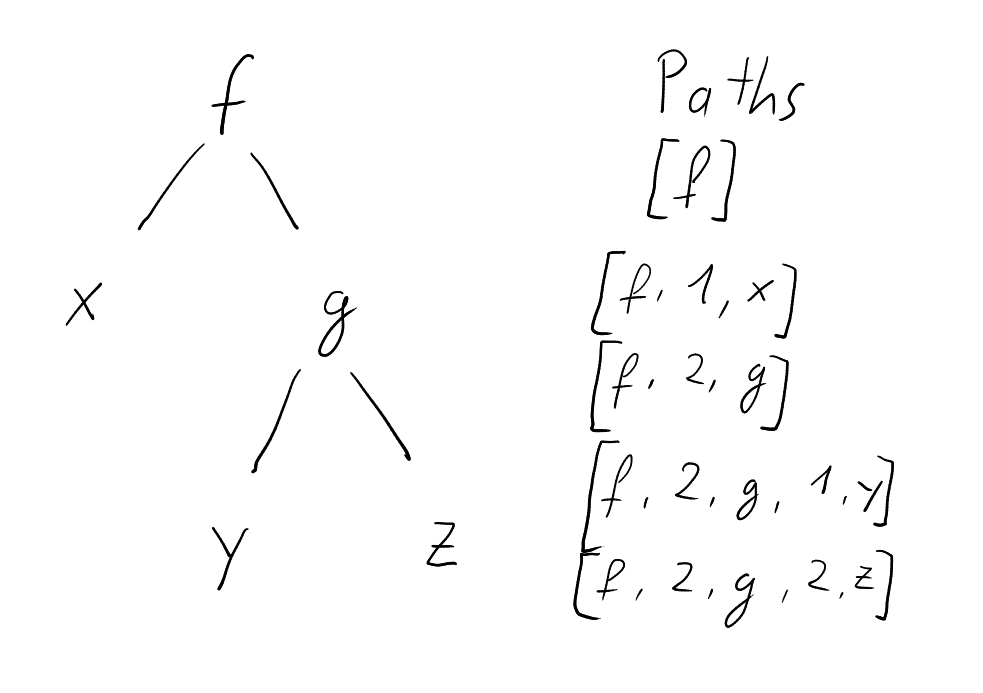
\includegraphics[scale=0.25]{figures/term_path.png}
\caption{A term and its paths together with the symbols associated with them}
\label{termpaths}
\end{figure}\todo{Write as mapping: $<> \longrightarrow f$ etc.}

A $(path, symbol)$ pair can be interpreted as a constraint on a term where the path defines the position of the symbol in the term. For example, $(<(f,1)>, c)$ is only fulfilled by terms of the form $f(c,...)$\footnote{The paths do not explicitly encode any information about the number of arguments.}. A term gives raise to a set of $(path, symbol)$ pairs, which, when interpreted as constraints, uniquely identify this term up to loss of variable identitification.

These constraints allow us to define terms not explicitly by their structure and symbols but rather by imposing constraints on them. This concept is fundamental to path indexing which stores only the constraints. Queries are resolved by combining the constraints to retrieve a set of terms.\todo{Better phrasing}

\begin{defn}
  A path index is a function $f: Path \times Symbol \longrightarrow 2^{Term}$, that is, each constraint is mapped to a set of terms, which fulfill these constraints and are stored in the path index. We call this set of terms a path set.\todo{Drop ``path set'' completely?}
\end{defn}

Storing the path sets such that they can be quickly looked up by a $(path, symbol)$ pair can be achieved in multiple ways. We decided to use a trie-based approach as many of the paths share prefixes. The nodes of the trie contain a function $g: Symbol  \longrightarrow 2^{Term}$. The edges are labelled with $(symbol, index)$ pairs, which correspond to the elements of a path. When we insert a path $p$ of a term $t$ we start at the root and traverse the trie according to $p$. Once we reach the end of $p$ we extend $g$ of the current node by $Symbol_{t}(p) \longrightarrow \{t\}$.\todo{If already existant: Expand set, else extend definition of g to $Symbol_{t}(p)$} To insert a term we simply insert all the paths that describe this term. This requires the insertion of many similar paths which profits from the prefix sharing.

\Cref{pathindex} shows a path index stored as a trie. The root contains a mapping from the symbol $f$ to both terms as they both share this constraint. In the first argument, reached by the edge $(f,1)$, the symbol $a$ is mapped only to the first term whereas $*$ is mapped to the second term. In the second argument, the terms share the constraint.
\begin{figure}[h]
\centering
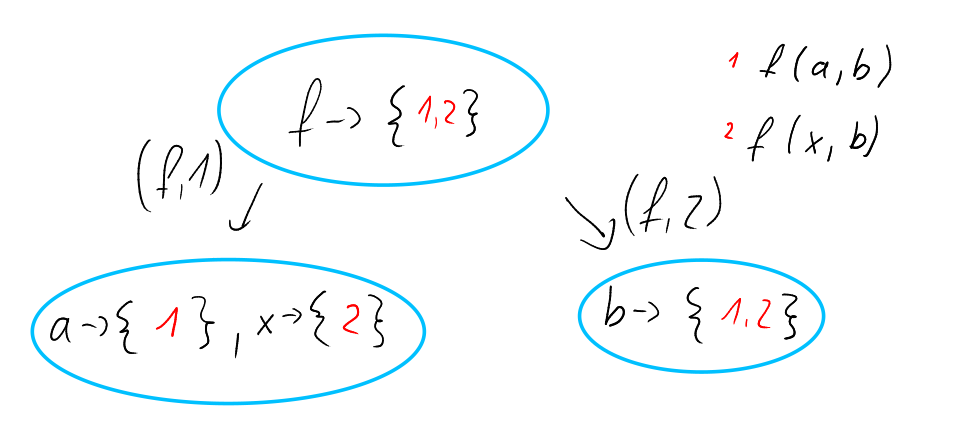
\includegraphics[scale=0.25]{figures/path_index.png}
\caption{A path index}
\label{pathindex}
\end{figure}

We are interested in retrieving the instances, generalisations and unifiables of a term stored in the index. In addition, we define a lookup to retrieve copies of the term. This can be used to check if a term is already contained but may also be of interest as different variables are not distinguished. The queries are based on intersections and unions of the different path sets to enforce constraints on the terms.

To answer the simplest query, the lookup, we procede as follows:
\begin{enumerate}
  \item Compute the set of $(path, symbol)$ pairs describing the term.
  \item Retrieve the path sets corresponding to them in the index.
  \item Intersect the path sets to retrieve all terms containing the same symbols at identical paths as the query term.
\end{enumerate}
  Under the assumption of consistent typing, we retrieve only terms of identical structure as $f(x,y)$ can not exist simultaneously to $f(x)$. Due to the loss of variable identity we may retrieve additional terms.

To retrieve the unifiables of a term from the index, we can use some observations regarding the unification problem.
\begin{enumerate}
  \item A variable is unifiable with any other term
  \item Constants are unifiable with themselves and variables
  \item A function $f(x_{1},...,x_{n})$ is unifiable with term $t$ if and only if $t = x$ or $t = f(y_{1},...,y_{n})$ where for all i $x_{i}$ is unifiable with $y_{i}$. Again, a differing number of arguments are impossible as their types would clash otherwise.
\end{enumerate}
Using this, we can define an algorithm recursing on the structure of the query term while intersecting and unifying the different path sets of the index. The different query types are quite similar, with the lookup being the most restrictive and the unifiables the least restrictive.

$\mathrm{PathTerms(p)}$ refers to the path set stored at the path $p$. $\mathrm{AllTerms}$ is the collection of all terms stored in the index.
\begin{figure}[h]
\centering
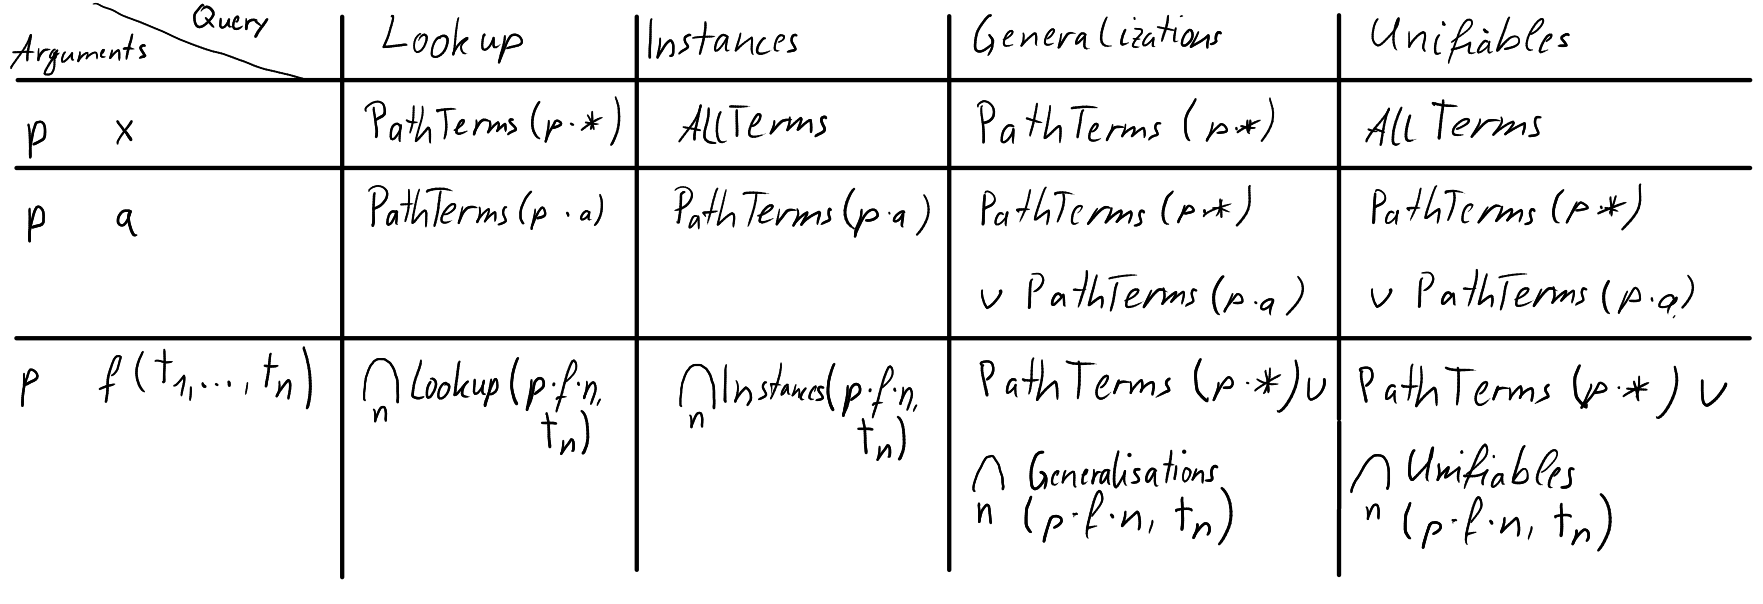
\includegraphics[scale=0.25]{figures/queries.png}
\caption{The different queries and their definition}
\end{figure}

\section{Implementation in Isabelle/ML}
The discrimination net implementation already present in Isabelle is used to store arbitrary values indexed by terms. This allows us to store certified terms or context together with terms. The lookup operation mentioned earlier is also more useful in this context.

Unfortunately most literature\todo{2 Quellen sicher, noch welche?} on path indexing only covers the storage of terms. The queries of path indexing rely on the intersection and union of path sets. These in turn rely on the fast comparison of the stored values. To solve this potential problem we investigated multiple solutions.

The first approach requires a comparison function for the values\footnote{Either as an argument to every function or by implementing path indexing as a functor on a value module}. Using the index becomes more difficult by doing so. A user has to implement a comparison function for values and additionally has to consider the potential performance impact. This can be partially mitigated by using $pointerEq$ although it can only be used as a shortcut for identical values, the comparison must still be called for differing values.

The second approach would be the storage of $(term, value)$ pairs. By doing so we can implement all the operations according to the literature and simply discard the term before returning the results. This simplifies implementation and retains acceptable performance as the comparison of differing values will likely only need to compare the first few symbols. It will also increase the memory consumption as a copy of every term is stored solely for the set operations. (Additionally there is no immutable pointer implementation in Isabelle/ML\todo{PolyML erwähnen?}. Instead, copies of identical values are shared by the runtime.)\todo{Überhaupt nicht erwähnen weil Data Sharing gut genug funktioniert?}

This approach can be further optimised by replacing the $(term, value)$ pairs by $(identifier, value)$ pairs and mapping each term to an identifier. By using integers as identifier we further speed up the comparison and can use ordered lists, provided by the SML standard library, for the path sets to implement the set operations more efficiently. We are also less reliant on the pointer equality provided by Poly/ML and runtime details like the merging of identical immutable values. This is quite important as we do not have any guarantee when the last heap compression occurred and manual invocation by using the ``shareCommonData'' introduces significant overhead to insertion. Additionally, reliance on low-level functions like ``shareCommonData'' and ``pointereq'' should be avoided as there are may be significant changes across runtime versions.

We can further speed up the set operations by building a tree of the intersections and unions and only evaluating it at the end. This likely utilizes the cache better because the previously calculated list is not evicted from the cache by the trie traversal. Furthermore, this presumably enables further compiler optimizations as the intermediate results are only short-lived and functions can be inlined.

Data Sharing in Poly/ML. NoConstraint exc. No generic hash. Saving ``Copy'' of values because pointers/ref are always mutable and bad for GC etc.
